\makeheading{Lecture 7 | 2020-09-28}
\section{Prediction}
Recall that $ \symbf{Y}=X\symbf{\beta}+\symbf{\varepsilon}
    \sim \text{MVN}(X\symbf{\beta},\sigma^2 I) $, and
\begin{itemize}
    \item Estimates: $ \hat{\symbf{\beta}}=(X^\top X)^{-1}X^\top \symbf{Y} $
    \item Fitted values: $ \hat{\symbf{\mu}}=X\hat{\symbf{\beta}} $
    \item Residuals: $ \symbf{e}=\symbf{y}-\hat{\symbf{\mu}} $
    \item Constants: $ X=\begin{bmatrix}
                  \symbf{1} & \symbf{x}_1 & \cdots & \symbf{x}_p
              \end{bmatrix}_{n\times(p+1)} $
    \item Values of responses: $
              \symbf{y}=(y_1,y_2,\ldots,y_n)^\top \in\mathbb{R}^n $
\end{itemize}

The span of $ X $ is $ \Span{X}=
    \set{b_0\symbf{1}+b_1\symbf{x}_1+\cdots+b_p\symbf{x}_p:b_0,\ldots,b_p\in\mathbb{R}}
    \subset \mathbb{R}^n $
which is all linear combinations of columns of $ X $ which is a subspace
of $ \mathbb{R}^n $, and by assumption we know $ \rank(X)=p+1 $.

We can say $ \Span{X} $ represents all possible vector
values $ X\symbf{b} $ where $ \symbf{b}=(b_0,b_1,\ldots,b_p)^\top $.

Generally, $ \symbf{y}\notin\Span{X} $, so since
the linear model is an approximation, $ \symbf{\varepsilon} $
variability not explained by model.

Intuitively, it makes sense to choose an estimate
$ \hat{\symbf{\beta}} $ so that $ X\hat{\symbf{\beta}} $
is as close to $ \symbf{y} $ as possible.

\begin{figure}[!htbp]
    \centering
    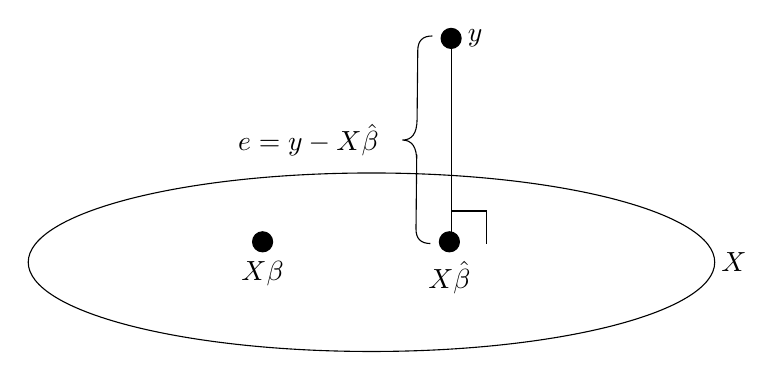
\begin{tikzpicture}[x=0.75pt,y=0.75pt,yscale=-1,xscale=1]
        %Shape: Ellipse [id:dp4907367451603444] 
        \draw   (5,122.67) .. controls (5,98.92) and (79.04,79.67) .. (170.38,79.67) .. controls (261.71,79.67) and (335.75,98.92) .. (335.75,122.67) .. controls (335.75,146.41) and (261.71,165.67) .. (170.38,165.67) .. controls (79.04,165.67) and (5,146.41) .. (5,122.67) -- cycle ;
        %Shape: Circle [id:dp31454130211800835] 
        \draw  [fill={rgb, 255:red, 0; green, 0; blue, 0 }  ,fill opacity=1 ] (203.92,14.83) .. controls (203.92,12.16) and (206.08,10) .. (208.75,10) .. controls (211.42,10) and (213.58,12.16) .. (213.58,14.83) .. controls (213.58,17.5) and (211.42,19.67) .. (208.75,19.67) .. controls (206.08,19.67) and (203.92,17.5) .. (203.92,14.83) -- cycle ;
        %Shape: Circle [id:dp6274550079547253] 
        \draw  [fill={rgb, 255:red, 0; green, 0; blue, 0 }  ,fill opacity=1 ] (113.08,112.83) .. controls (113.08,110.16) and (115.25,108) .. (117.92,108) .. controls (120.59,108) and (122.75,110.16) .. (122.75,112.83) .. controls (122.75,115.5) and (120.59,117.67) .. (117.92,117.67) .. controls (115.25,117.67) and (113.08,115.5) .. (113.08,112.83) -- cycle ;
        %Straight Lines [id:da5333534031755512] 
        \draw    (209,20) -- (209,114) ;
        %Shape: Circle [id:dp15834130769816157] 
        \draw  [fill={rgb, 255:red, 0; green, 0; blue, 0 }  ,fill opacity=1 ] (203.08,112.83) .. controls (203.08,110.16) and (205.25,108) .. (207.92,108) .. controls (210.59,108) and (212.75,110.16) .. (212.75,112.83) .. controls (212.75,115.5) and (210.59,117.67) .. (207.92,117.67) .. controls (205.25,117.67) and (203.08,115.5) .. (203.08,112.83) -- cycle ;
        %Shape: Brace [id:dp31280695059289887] 
        \draw   (199.75,13.67) .. controls (195.08,13.62) and (192.73,15.93) .. (192.68,20.6) -- (192.35,53.87) .. controls (192.28,60.54) and (189.92,63.85) .. (185.25,63.8) .. controls (189.92,63.85) and (192.22,67.2) .. (192.15,73.87)(192.18,70.87) -- (191.83,106.6) .. controls (191.78,111.27) and (194.09,113.62) .. (198.76,113.67) ;
        %Shape: Right Angle [id:dp8084265870567517] 
        \draw   (209,98) -- (226,98) -- (226,114) ;
        % Text Node
        \draw (337.75,122.67) node [anchor=west] [inner sep=0.75pt]    {$\Span{X}$};
        % Text Node
        \draw (117.92,121.07) node [anchor=north] [inner sep=0.75pt]    {$X\symbf{\beta}$};
        % Text Node
        \draw (207.92,121.07) node [anchor=north] [inner sep=0.75pt]    {$X\hat{\symbf{\beta}}$};
        % Text Node
        \draw (215.58,14.83) node [anchor=west] [inner sep=0.75pt]    {$\symbf{y}$};
        % Text Node
        \draw (140,55) node [anchor=north] [inner sep=0.75pt]    {$\symbf{e}=\symbf{y}-X\hat{\symbf{\beta}}$};
    \end{tikzpicture}
\end{figure}


Therefore, $ \symbf{e} $ must be orthogonal to $ \Span{X}
    \iff \symbf{e} $ is orthogonal to all columns of $ X $.
\begin{align*}
    \symbf{1}^\top(\symbf{y}-\hat{\symbf{\mu}})   & =       0 \\
    \symbf{x}_1^\top(\symbf{y}-\hat{\symbf{\mu}}) & =       0 \\
                                                  & \vdots    \\
    \symbf{x}_p^\top(\symbf{y}-\hat{\symbf{\mu}}) & =       0
\end{align*}
which is the same as LS estimates. We also know
$ \hat{\symbf{\mu}}=X\hat{\symbf{\beta}} $ and
$ \symbf{e}=\symbf{y}-\hat{\symbf{\mu}} $.
\begin{Definition}{Hat matrix}{}
    The \textbf{hat matrix} is defined as
    $ H=X(X^\top X)^{-1}X^{\top} $.
\end{Definition}

\begin{Proposition}{Properties of Hat Matrix}{hat_prop}
    Let $ H $ be a hat matrix, then $ H $ has the following properties.
    \begin{enumerate}[label=(\arabic*)]
        \item $ H $ is symmetric; that is, $ H=H^\top $.
        \item $ H $ is idempotent; that is, $ H^2=HH=H $.
        \item $ I-H $ is symmetric idempotent; that is,
              $ (I-H)^2=(I-H)(I-H)=I-H $.
    \end{enumerate}
\end{Proposition}
\begin{Proof}{\ref{prop:hat_prop}}{} We prove all three because it's easy.
    \begin{enumerate}[label=(\arabic*)]
        \item $ H^\top=[X(X^\top X)^{-1}X^\top]^\top=X(X^\top X)^{-1}X^\top=H $.
        \item  $ HH=X(X^\top X)^{-1}(X^\top X)(X^\top X)^{-1}X^\top=H $.
        \item  $ (I-H)(I-H)=I(I-H)-H(I-H)=II-IH-HI+HH=I-2H+HH=I-2H+H=I-H $.
    \end{enumerate}
\end{Proof}
Let's view $ \hat{\symbf{\mu}} $ and $ \symbf{e} $
as random vectors
\[ \hat{\symbf{\mu}}=X\hat{\symbf{\beta}}=
    X(X^\top X)^{-1}X^\top \symbf{Y}=H\symbf{Y} \]
\[ \symbf{e}=\symbf{Y}-\hat{\symbf{\mu}}=I\symbf{Y}-H\symbf{Y}=
    (I-H)\symbf{Y} \]
\[ \E{\hat{\symbf{\mu}}}=\E{H\symbf{Y}}=H\E{\symbf{Y}}=
    X(X^\top X)^{-1}X^\top \Uunderbracket{X\symbf{\beta}}_{\E{\symbf{Y}}}
    =X\symbf{\beta}
\]
\[ \Var{\hat{\symbf{\mu}}}=\Var{H\symbf{Y}}=
    H\Var{\symbf{Y}}H^\top=H\sigma^2I H^\top=\sigma^2(H H^\top)=\sigma^2H \]
\[ \E{ \symbf{e}}=
    \E{(I-H)\symbf{Y}}=\E{\symbf{Y}}-\E{H\symbf{Y}}=X\symbf{\beta}-X\symbf{\beta}=0 \]
\[ \Var{\symbf{e}}=
    (I-H)\Var{\symbf{Y}}(I-H)^\top=\sigma^2(I-H)(I-H)^\top=\sigma^2(I-H) \]
So since $ \hat{\symbf{\mu}} $ and $ \symbf{e} $
are linear transformations of $ \symbf{Y} $ we have proved the following theorem.
\begin{Theorem}{Distribution of $ \hat{\symbf{\mu}} $ and $ \symbf{e} $}{}
    $ \hat{\symbf{\mu}} $ and $ \hat{\symbf{e}} $ have the following distribution.
    \[ \hat{\symbf{\mu}}\sim\text{MVN}(X\symbf{\beta},\sigma^2 H) \]
    \[ \hat{\symbf{e}}\sim\text{MVN}(0,\sigma^2(I-H)) \]
\end{Theorem}
Suppose we want to predict response for $ \symbf{x}_0 $
where the first 1 represents the intercept in the row vector.
\[ \symbf{x}_0=\begin{bmatrix}
        1 & x_{01} & x_{02} & \cdots & x_{0p}
    \end{bmatrix}_{1\times (p+1)} \]
Let $ Y_0 $ random variable representing the response
associated with $ \symbf{x}_0 $. In multiple linear regression,
\[ Y_0 \sim \N{\beta_0+\beta_1x_{01}+\cdots+\beta_p x_{0p},\sigma^2} \]
So we predict the value
\[ \hat{y}_0=\hat{\beta}_0+\hat{\beta}_1x_{01}+\cdots+
    \hat{\beta}_p x_{0p}=\symbf{x}_0\hat{\symbf{\beta}} \]
which represents the estimated mean response given
$ x_{01},x_{02},\ldots,x_{0p} $. Corresponding distribution
has
\[ \E{\hat{Y}_0}=\symbf{x}_0\E{\hat{\symbf{\beta}}}=\symbf{x}_0\symbf{\beta}
    =\E{Y_0} \]
\[ \Var{\hat{Y}_0}=\symbf{x}_0\Var{\hat{\symbf{\beta}}}\symbf{x}_0^\top=
    \symbf{x}_0\sigma^2(X^\top X)^{-1}\symbf{x}_0^\top \]
We have proved the following theorem.
\begin{Theorem}{Distribution of Predictor}{}
    The distribution of $ \hat{Y}_0 $ which is a function
    of $ Y_1,\ldots,Y_n $ is
    \[ \hat{Y}_0 \sim \N{\symbf{x}_0\symbf{\beta},\sigma^2\symbf{x}_0(X^\top X)^{-1}
            \symbf{x}_0^\top} \]
\end{Theorem}
\[ \frac{\hat{Y}_0-\symbf{x}_0\symbf{\beta}}{\sigma\sqrt{
            \symbf{x}_0(X^\top X)^{-1}\symbf{x}_0^\top
        }}\sim \N{0,1}  \]
\[ \frac{\hat{Y}_0-\symbf{x}_0\symbf{\beta}}{\hat{\sigma}\sqrt{
            \symbf{x}_0(X^\top X)^{-1}\symbf{x}_0^\top
        }}\sim t(n-(p+1))=t(n-p-1)  \]
A $ (1-\alpha) $ confidence interval for the mean
response $ y_0=\symbf{x}_0\hat{\symbf{\beta}} $ given $ \symbf{x}_0 $ is
\[ \hat{y}_0\pm c \hat{\sigma}\sqrt{
        \symbf{x}_0(X^\top X)^{-1}\symbf{x}_0^\top} \]
where $ c $ is the $ 1-\alpha/2 $ quantile of $ t(n-p-1) $.

Prediction error: $ Y_0-\hat{Y}_0 $ which are independent
since $ Y_0 $ is a random variable with variance $ \sigma^2 $
and $ \hat{Y}_0 $ is a function of $ Y_1,\ldots,Y_n $. Therefore,
\[ \E{Y_0-\hat{Y}_0}=\symbf{x}_0\symbf{\beta}-\symbf{x}_0\symbf{\beta}=0 \]
\[ \Var{Y_0-\hat{Y}_0}=\Var{Y_0}+(-1)^2\Var{\hat{Y}_0}=
    \sigma^2+\sigma^2(\symbf{x}_0(X^\top X)^{-1}\symbf{x}_0^\top) \]
We have proved the following theorem.
\begin{Theorem}{Distribution of Prediction Error}{}
    The distribution of the prediction error is
    \[ Y_0-\hat{Y}_0 \sim N(
        0,\sigma^2(1+\symbf{x}_0(X^\top X)^{-1}\symbf{x}_0^\top)). \]
\end{Theorem}

A $ (1-\alpha) $ prediction interval for the mean
response $ y_0=\symbf{x}_0\hat{\symbf{\beta}} $ given $ \symbf{x}_0 $ is
\[ \hat{y}_0\pm c\hat{\sigma}\sqrt{1+\symbf{x}_0(X^\top X)^{-1}\symbf{x}_0^\top} \]
where $ c $ is the $ 1-\alpha/2 $ quantile of $ t(n-p-1) $.

\begin{Remark}{}{}
    Our intuition tells us that the prediction interval is wider than
    the confidence interval for mean. In other words, estimating
    an average is ``easier'' than an individual response.
\end{Remark}
